%==============================================================================
\section{Introdu\c{c}\~{a}o}
\label{sec:introducao}
%==============================================================================
	
%Inicie aqui o texto da sua introdução. As referências devem ser feitas utilizando o codigo a seguir~\cite{Ermagan08}

%Uma figura é inserida no texto da seguinte forma: A Figura~\ref{fig:sample-eai-solution} representa ...

%\begin{figure}
%    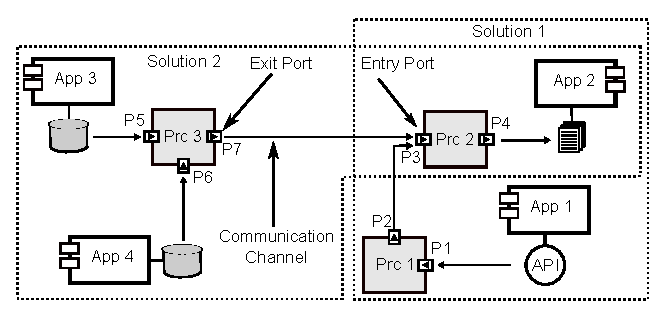
\includegraphics[scale=0.7]{./figs/sample-solution.eps}
%   \caption{Sample EAI solutions.}
%    \label{fig:sample-eai-solution}
%\end{figure}
%-- Context
%A Integração de Aplicações Empresariais (EAI) é o campo de estudo que proporciona metodologias, técnicas e ferramentas para a 
\noindent 
%--Context
As empresas possuem um ecossistema de software composto por diversas aplicações que geralmente são desenvolvidas internamente ou adquiridas de terceiros. O avanço das tecnologias de desenvolvimento de aplicações e a incorporação de serviços de software disponíveis na internet têm deixado os ecossistemas de software ainda mais heterogêneos. Os processos de negócio de uma empresa precisam ser suportados por um conjunto de aplicações e serviços de software que integram seu ecossistema, porém, frequentemente, tais aplicações e serviços não estão preparados para trabalhar de forma conjunta. A Integração de Aplicações Empresariais (EAI) é o campo de estudo que oferece metodologias, técnicas e ferramentas para que os processos de negócio funcionem de forma sincronizada, promovendo repostas rápidas e confiáveis.  

%--Problem
As plataformas de integração são softwares especializados que permitem projetar, executar e monitorar soluções de integração, as quais conectam funcionalidades e dados de diferentes aplicações. Uma solução de integração implementa um fluxo de integração composto por distintas tarefas atômicas que são executadas ao longo desse fluxo. Gregor Hophe e Bobby Woolf~\cite{hohpe2004} documentaram um conjunto de padrões de integração que tem inspirado o desenvolvimento de plataformas de integração de código aberto e que por sua vez organizam o fluxo de integração seguindo uma arquitetura Pipes\&Filters~\cite{alexander1977}. 
%Dentre essas plataformas, destacam-se Camel~\cite{isen2010}, Spring~\cite{fisher2012}, Mule~\cite{dossot2014}, Guaraná~\cite{frantz2016}, Jitterbit~\cite{russell2012} e
% WSO2 ESB~\cite{indrasiri2016}. 
 Usualmente, essas plataformas fornecem uma linguagem de domínio específico, um kit de ferramentas de desenvolvimento, um motor de execução e uma ferramenta de monitoramento. A linguagem de domínio específico possibilita a descrição de modelos conceituais para soluções de integração. O kit de desenvolvimento é um conjunto de ferramentas de software que permite a implementação de soluções, ou seja, transforma uma solução conceitual em código executável. O motor proporciona todo o suporte necessário à execução das soluções de integração. A ferramenta de monitoramento é utilizada para detectar erros que possam ocorrer durante a execução de soluções de integração. O motor é o responsável pela execução das soluções de integração~\cite{frantz2016}. 

As tarefas da solução de integração são executadas por meio de recursos computacionais presentes no motor de execução, dentre os quais estão as \emph{threads} de execução. Neste contexto, as \emph{threads} s\~{a}o usadas para proporcionar que as tarefas sejam executadas de forma simultânea, por meio da programação \emph{multithreads}~\cite{dietel2009,tanebaum2009}. Nesse tipo de programação, a criação de \emph{threads} pode impactar o desempenho da execução de uma solução de integração.

%-- Why it is a problem
Um algoritmo de agendamento de tarefas inadequado aumenta o tempo de execução, impactando o desempenho da solução de integração. A abordagem mais comum é a contratação de mais recursos computacionais, porém essa alternativa é financeiramente onerosa e nem sempre viável. Nossa revisão da literatura identificou que os motores de integração adotam como política de agendamento de tarefas as políticas de prioridade e a \textit{First-In-First-Out} (FIFO). Há propostas de algoritmos de agendamento de tarefas para máquina virtuais em sistemas distribuídos~\cite{rodriguez2014,al2015}, porém não foram identificadas propostas que foquem na otimização de desempenho de motores de execução de plataformas de integração de sistemas. 
%
% O agendamento de fluxo de trabalho tem sido amplamente estudado ao longo dos anos, nos quais os algoritmos se concentram na geração de soluções aproximadas ou quase ótimas, por se tratar de um problema não polinomial difícil~\cite{sousa2004}. Pandey et al.~\cite{pandey2010} propõem um algoritmo baseado em PSO para minimizar o custo de execução de um único fluxo de trabalho enquanto equilibra a carga da tarefa nos recursos disponíveis. Wu et al.~\cite{wu2010} usam PSO para produzir um agendamento quase ideal, se preocupando em minimizar custo e tempo, mas assume que um conjunto limitado de recursos, sem levar em conta a elasticidade proporcionada com a computação em das nuvens. O algoritmo de Byun et al.~\cite{byun2011} estima o número ótimo de recursos que precisam ser alocados para que o custo de execução de um fluxo de trabalho seja minimizado. Sua abordagem aproveita a elasticidade dos recursos da nuvem, mas não considera a natureza heterogênea dos recursos computacionais.

A contribuição deste trabalho é a aplicação da meta-heurística \textit{Particle Swarm Optimization} (PSO) para o contexto dos motores de execução, nos quais as políticas de agendamento adotadas, não consideram o tempo de espera na fila de tarefas prontas, nem a complexidade computacional das tarefas. PSO é fácil de implementar e existirem poucos parâmetros para serem ajustado, adequando-se ao problema de encontrar melhor agendamento das tarefas. Classifica-se como uma pesquisa exploratória, a medida que busca um método mais eficiente do que os existentes, na resolução do problema. Um resumo com ideias iniciais para esse trabalho foi apresentado em um seminário de pesquisa~\cite{sellaro2017}, e o presente artigo as discute de forma mais ampla e completa  a proposta de um algoritmo que busca o mapeamento ótimo das tarefas para os pools de \emph{threads}.

%-- Solution
O resto deste artigo está organizado como segue. A Seção 2 apresenta a formulação do problema. A Seção 3 descreve sucintamente a técnica PSO. A Seção 4 expõe a abordagem proposta. E a Seção 5 apresenta nossas conclusões e perspectivas de trabalhos futuros. 